\documentclass[12pt]{article}

\usepackage[english]{babel}
\usepackage[letterpaper,top=2cm,bottom=2cm,left=2cm,right=2cm,marginparwidth=1.75cm]{geometry}

\usepackage{amsmath}
\usepackage{amsthm}
\usepackage{amsfonts}
\usepackage{graphicx}
\usepackage{float}

\title{Complex graph properties and their use in the real world}
\author{Zi Chen}
\date{}

\begin{document}
\maketitle

\section{Introduction}
The application of mathematics have played a key role in the development of technological advancements and breakthroughs in sciences. Throughout history, it has provided us with an increasing amount of various branches such as discrete maths, applied maths, cartesian geometry, algebra, calculus and many more. All of which can be applied to the real world, whether it is for construction, physics or day to day life. A key branch under discrete mathematics is graph theory where models can be developed to represent relations between different objects. Graphs has a range of uses both in the mathematical world and the real world. They can be used to represent large sets of data visually so that different information can be derived from the graph such as clustering of certain areas, the connectiveness between vertices or edges and what these may correlate to. These are the areas that I will explore and a way to visualise them by using python. They are also widely known as networks with some examples such as a friendship network, business networks and even a food chain level.

Graph theory was first introduced in 1736 from a solution to the seven bridges of Kongisberg. This famous problem 

Examples of what they can represent ranges from simple relationships between people to the complex structure of the brain. Once a mathematical structure, which can be called a graph or network, is created as a basis of representation of relations, various patterns and correlations can be derived to generate graph properties that can later be used to develop useful information and possible improvements to the whole graph.  
\\

By using vertices and edges, which can carry weights and be directed, we can visually represent a graph. They can also be represented by adjacency matrices. Within this matrix holds the values of each edge known as its weight and where it's located will decide the start and end of the edge as the rows and columns are the vertices for this graph. This means that by analysing the graph we are able to generate numerical values representing certain factors of the graph. Which can then further be used to display the network so that further correlation can be identified.

\section{Property Visualisation}
Initially I explored the trophic coherence\cite{1} which determines the stability and how well their trophic levels work. Trophic levels are taken from ecology and applied to graphs to generate a height based format for the vertices of a graph. For a graph $G =(V,E)$ (can be directed), we have $V$ which is the set of all vertices in $G$ and $E$ which is the set of all the edges within $G$. Each edge can carry a weight between a vertex $u$ to a vertex $v$, however if the graph isn't weighted then the value is 1 if an edge exists. Thus, the graph can be represented as an adjacency matrix $W$ which incorporates the direction of the edges, whether if its a loop and the weight of the edges if applicable or 1 otherwise. We can define the total weight (also known as the strength) for each vertex by the weights into a vertex $u$ and the weights out of vertex $u$, which is shown by $s_v$. The imbalance of the vertex $u$ by the weights in minus the weights out shown by $i_v$.
$$ s_v = \sum(w_{uv}) + \sum(w_{vu}),\qquad i_v = \sum(w_{uv}) - \sum(w_{vu})$$
Vectors $s$ and $i$ holds all the values of the strength and imbalance for all vertices respectively. We let $h$ be a vector, then the graph laplacian operator in matrix form is defined by
$$\Delta = \text{diag}(u) - W - W^T$$
Therefore to get the trophic levels for each vertex, we solve the system of equations for vector $h$.
$$\Delta h = v $$
The values within this vector can be used to illustrate the various trophic levels\cite{2} within a graph. 
\\

An additional property in graphs is the clustering coefficient $C$ which quantifies the probability of a vertex $a$ having an edge to vertex $c$ if $ab$,$bc \in E(G)$. There are 2 types, the local clustering coefficient and the global clustering coefficient\cite{3}. The global clustering coefficient $C$ for both undirected and directed graphs can be defined as 
$$ C = \frac{3\text{(Number of total triangles)}}{\text{Number of total connected triples}} $$
The local clustering coefficient $C_i$ measures how close the neighbours of a vertex are being to a complete graph (a clique). The definition of $C_i$ for a directed graph is given by
$$ C_i = \frac{\text{Number of triangles connected to $i$}}{\text{Number of triples centered on vertex $i$}}$$
If the graph is undirected then the possible triples that is centered on a vertex $i$ is half of when they were directed as the in edge can also be an out edge for $i$ as they are directionless. So the clustering coefficient can be defined as 
$$ C_i = \frac{2\text{(Number of triangles connected to $i$)}}{\text{Number of triples centered on vertex $i$}}$$
Another way to represent the global clustering coefficient is to take the averages of all the local coefficients. When the vertices have a degree of 0 or 1 then $C_i = 0$ so clustering coefficient is 
$$ C = \frac{1}{n}\sum_i{C_i}i$$
So that we can visualise the coefficients, I've focused on the local clustering coefficients as these are for individual vertices rather than the graph as a whole.
\\
Betweenness centrality\cite{4} measures the centrality of a graph by using shortest paths. The higher the value for a vertex, the greater the connections to other vertices as a shortest path. In other words, if the value is large then for a vertex, then the travel time from this vertex to other vertices is shorter. The calculation for each vertex $u$ is determined from 
$$ G(u)=\sum_{a\ne u\ne b}\frac{P_{ab}(u)}{P_{ab}}$$
where $P_{ab}(u)$ is the number of shortest paths from vertex $a$ to vertex $b$ that includes vertex $u$ but not as an end point. $P_{ab}$ is the total number of shortest paths from vertex $a$ to vertex $b$.
\begin{figure}[H]
	\centering
	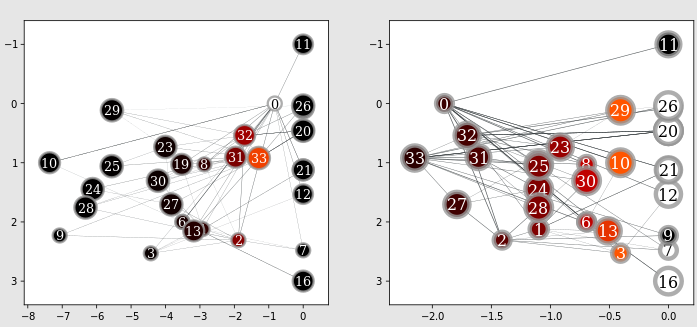
\includegraphics[width=\linewidth]{graphs.jpg}
	\caption{A graph generated by a dataset representing karate clubs and their relations. Both graphs have their y-axis as the tropic coherence values. The left graph has betweenness 			centrality as the x-axis and the right has their clustering coefficients plotted on the x-axis.}
	\label{fig:graph}
\end{figure}
Therefore by taking these properties, the graph can be rearranged in accordance to their values. This is accomplished by having their property values as their position vector. In our case we have trophic levels as the y-axis and the clustering coefficients or betweenness centrality as the x-axis shown on Figure \ref{fig:graph}.
\section{Future aims}
I will continue experimenting with these properties and to research other values that may provide a greater insight for the graphs. Another aim is to use various types of data sets and find any correlation or patterns between their properties. These data sets will be taken from real world networks such as business networks, club networks etc. There is also the use of the properties by other means rather than using a graph comparison. An example for this is the clustering coefficient where they can be used to plot a network that represents the brain which will lead to certain areas clustering as the neurons\cite{5} within a brain would. Furthermore this can be used on patients with Alzheimer's to see if the clustering coefficients vary among them. I will also read and research other areas relating to properties of graphs.

\bibliographystyle{alpha}
\bibliography{sample}

\begin{thebibliography}{9}
\bibitem{1}
MacKay RS, Johnson S, Sansom B. 2020 How directed is a directed network? R. Soc. Open Sci. 7: 201138. http://dx.doi.org/10.1098/rsos.201138
\bibitem{2}
Samuel Johnson 2020 Digraphs are different: why directionality matters in complex systems J. Phys. Complex. 1 015003
\bibitem{3}
Newman, 2003, The Structure and Function of Complex Network, https://doi.org/10.48550/arXiv.cond-mat/0303516
\bibitem{4}
Ulrik Brandes, Stephen P. Borgatti, Linton C. Freeman, Maintaining the duality of closeness and betweenness centrality, https://doi.org/10.1016/j.socnet.2015.08.003
\bibitem{5}
Matthew R. Brier, Jewell B. Thomas, Anne M. Fagan, Jason Hassenstab, David M. Holtzman, Tammie L. Benzinger, John C. Morris, Beau M. Ances, Functional connectivity and graph theory in preclinical Alzheimer's disease, Neurobiology of Aging, Volume 35, Issue 4, 2014, https://doi.org/10.1016/j.neurobiolaging.2013.10.081
\end{thebibliography}

\end{document}